%%%%%%%%%%%%%%%%%%%%%%%%%%%%%%%%%%%%%%%%%%%%%%%%%%%%
%
% Copyright 2022 
%
% This file may be distributed and/or modified
%
% 1. under the LaTeX Project Public License and/or
% 2. under the GNU Public License.
%
%%%%%%%%%%%%%%%%%%%%%%%%%%%%%%%%%%%%%%%%%%%%%%%%%%%%%%%%%%%

%%%   DESCRIZIONE 

% Non riuscendo a trovare un tema per la classe Beamer che mi soddisfacesse, 
% ho provveduto alla creazione del seguente tema che ho utilizzato per la realizzazione 
% della presentazione che ha accompagnato la discussione di tesi di laurea. 
% Il tema è basato a partire dal colore blu del logo dell'università degli
% studi di Trieste, dal quale è stata creata una palette di colori aggiungendo 
% gradualmente del bianco. 
% 
%  Nota:  
% Per il caso specifico (discussione di tesi) in cui mi è servito il tema, ho impostato ad hoc
% una disposizione alternativa del primo frame rispetto a quello che si otterrebbe normalmente 
% con il comando \maketitle. 
% Per evitare questo basta commentare il comando \setTitlestyleDissertation immediatamente precedente. 
%
% Il layout proposto potrebbe essere leggermente rivisto, per es. nel caso in cui fosse 
% presente anche un correlatore. In questo bisogna decommentare nel file:
%		otherResources/presentazione_myThemeSetting.tex
% le opportune linee di codice dove suggerito. 
% Sempre agendo nel suddetto file è possibile anche impostare il layout utilizzando solamente 
% il logo dell'università, omettendo quindi il logo del dipartimento. In generale da tale 
% file è possibile apportare qualisasi modifica al tema. Consiglio di consultare la 
% documentazione del paccehtto beamer all'indirizzo: 
%	https://mirror.math.princeton.edu/pub/CTAN/macros/latex/contrib/beamer/doc/beameruserguide.pdf

\documentclass{beamer}

% Caricamento di tutti i pacchetti necessari 
\usepackage{presentation/setting/packages}
%\setbeamersize{text margin left=5mm,text margin right=5mm} 

\newcommand*\circled[1]{\tikz[baseline=(char.base)]{
    \node[shape=ellipse,draw=red,inner sep=1.5pt] (char) {#1};}}





% Settaggi documento %%
        
\hypersetup{
    pdfauthor={Nome Cognome},
    pdftitle={Titolo presentazione},
    pdfsubject={Argomento presentazione}
}
\title[]{Characterization of monolithic CMOS pixel sensors for charged particle detectors and for high intensity dosimetry}

\institute{Università degli studi di Pisa}
\author[Eleonora Ravera]{Eleonora Ravera}
\year=2022
\month=10
\day=27
\def\relatore{Francesco Forti}
\def\relatoreLabel{Supervisors:}
\def\correlatore{Maria Giuseppina Bisogni}
\def\correlatoreLabel{Co-supervisor:}
\def\candidatoLabel{Candidate:}
\def\LogoUniversita{figures/Logo-UNIPisa.png}
%\def\LogoFiligrana{otherResources/background-blu.png}

%Applico tutte le personalizzazioni desiderate al tema: 
%%%%%%%%%%%%%%%%%%%%%%%%%%%%%%%%%%%%%%%%%%%%%%%%%%%%%%%%%%%
%
% Copyright 2022 by Isac Pasianotto
%
% This file may be distributed and/or modified
%
% 1. under the LaTeX Project Public License and/or
% 2. under the GNU Public License.
%
%%%%%%%%%%%%%%%%%%%%%%%%%%%%%%%%%%%%%%%%%%%%%%%%%%%%%%%%%%%
\setbeamertemplate{navigation symbols}{}

%% 	Variabili di tipo "color": 

\definecolor{bluUnits100}{rgb}{0.16,0.22,0.36} 
\definecolor{bluUnits80}{rgb}{0.22,0.3,0.51}
\definecolor{bluUnits70}{rgb}{0.25,0.35,0.58}
\definecolor{bluUnits50}{rgb}{0.41,0.51,0.74}
\definecolor{bluUnits40}{rgb}{0.56,0.63,0.81}
\definecolor{bluUnits25}{rgb}{0.78,0.82,0.9}
\definecolor{bluUnits10}{rgb}{0.93,0.94,0.96}
\definecolor{grey}{rgb}{0.3686, 0.5255, 0.6235} 
%\definecolor{celadon}{rgb}{0.67, 0.88, 0.69}
\definecolor{celadon}{rgb}{0.67, 0.93, 0.79}
\definecolor{gray}{rgb}{0.8, 0.8, 0.8}


%%	Palette di colori 

\setbeamercolor{palette primary}{bg=bluUnits100,fg=white}
\setbeamercolor{palette secondary}{bg=bluUnits80,fg=bluUnits25}
\setbeamercolor{palette tertiary}{bg=bluUnits50,fg=bluUnits100}
\setbeamercolor{palette quaternary}{bg=bluUnits40,fg= bluUnits100}
\setbeamercolor{palette quaternary blue}{bg=bluUnits40,fg=bluUnits100}
\setbeamercolor{palette light primary}{bg=bluUnits25,fg=bluUnits100}
\setbeamercolor{palette titleframe}{bg=bluUnits10, fg=bluUnits80}

\setbeamercolor{celadon}{bg=celadon, fg=bluUnits80}
\setbeamercolor{gray}{bg=gray, fg=bluUnits80}


		%%%%%%%%%%%%%%%%%%%%%%%%%%%%%%%%%%
		%% Impostazioni generali slide  %%
		%%%%%%%%%%%%%%%%%%%%%%%%%%%%%%%%%%

%%	Setta l'immagine da mettere come sfondo, riducendone l'opacità
%\usebackgroundtemplate{\tikz\node[opacity=0.1]{\includegraphics[height=\textheight]{\LogoFiligrana}};}

%%	Elenchi puntati, numerati, etc.
\setbeamercolor{structure}{fg=bluUnits80}
\setbeamertemplate{enumerate item}[circle]
\setbeamertemplate{itemize subitem}[ball]
% Valutare a secoda del contesto se sostituire con 
%\setbeamertemplate{items}[circle]
\setbeamertemplate{items_circ}[circle]
\setbeamercolor{alerted text}{fg=bluUnits50}

%% 	Colore delle scritte nella presentazione
\setbeamercolor{normal text}{fg=bluUnits100,bg=white}

		%%%%%%%%%%%%%%%%%%%%%%%%%%%%%%%%%%
		%% Impostazioni normal slides  %%
		%%%%%%%%%%%%%%%%%%%%%%%%%%%%%%%%%%
%% 	Settaggio della linea in alto (headline)
\setbeamertemplate{headline}{
	\vskip1pt
	\leavevmode	
	\hbox{
		\begin{beamercolorbox}[wd=.99\paperwidth,ht=2.5ex,dp=1.125ex]{palette light primary}
			\insertsectionnavigationhorizontal{\paperwidth}{\hskip0pt plus1fill}{\hskip0pt plus1fill}
		\end{beamercolorbox}
	}
}

%%	Settaggio riga in basso (footline) 
\setbeamertemplate{footline}{
       \leavevmode
	   \hbox{
           \begin{beamercolorbox}[wd=.2\textwidth,ht=2.6ex,dp=1ex,center]{palette tertiary}
		    \usebeamerfont{date in head/foot}\insertdate
    	\end{beamercolorbox}
	
    	\begin{beamercolorbox}[wd=.27\textwidth,ht=2.6ex,dp=1ex,center]{palette quaternary}
	   		\usebeamerfont{author in head/foot}\insertshortauthor
	   	\end{beamercolorbox}
	
    	\begin{beamercolorbox}[wd=.4\textwidth,ht=2.6ex,dp=1ex,center]{palette primary}
    		\usebeamerfont{institute in head/foot}\insertshortinstitute
    	\end{beamercolorbox}

    	\begin{beamercolorbox}[wd=.1\textwidth,ht=2.6ex,dp=1ex,center]{palette light primary}
	   		\insertframenumber{}/\inserttotalframenumber\strut\quad
	    \end{beamercolorbox}
    }
    \vskip2pt

}

%%	Settaggio tittoli delle slide  
\setbeamertemplate{frametitle}{
	\begin{beamercolorbox}[wd=\paperwidth,ht=2.75ex,dp=1ex,left]{palette titleframe}
		\qquad \textbf{\insertframetitle}
	\end{beamercolorbox}
}



		%%%%%%%%%%%%%%%%%%%%%%%%%%%%%%%%%%
		%% Impostazioni backup slides  %%
		%%%%%%%%%%%%%%%%%%%%%%%%%%%%%%%%%%
%% 	Settaggio della linea in alto (headline)
\defbeamertemplate{headline}{backup}{
	\vskip1pt
	\leavevmode	
	\hbox{
		\begin{beamercolorbox}[wd=.99\paperwidth,ht=2.5ex,dp=1.125ex]{palette light primary}
		\end{beamercolorbox}
	}}

%%	Settaggio riga in basso (footline) 
\defbeamertemplate{footline}{backup}{
       \leavevmode
	   \hbox{
           \begin{beamercolorbox}[wd=.2\textwidth,ht=2.6ex,dp=1ex,center]{palette tertiary}
		    \usebeamerfont{date in head/foot}\insertdate
    	\end{beamercolorbox}
	
    	\begin{beamercolorbox}[wd=.27\textwidth,ht=2.6ex,dp=1ex,center]{palette quaternary}
	   		\usebeamerfont{author in head/foot}\insertshortauthor
	   	\end{beamercolorbox}
	
    	\begin{beamercolorbox}[wd=.4\textwidth,ht=2.6ex,dp=1ex,center]{palette primary}
    		\usebeamerfont{institute in head/foot}\insertshortinstitute
    	\end{beamercolorbox}

    	\begin{beamercolorbox}[wd=.1\textwidth,ht=2.6ex,dp=1ex,center]{palette light primary}
	    \end{beamercolorbox}
    }
    \vskip2pt
}


		%%%%%%%%%%%%%%%%%%%%%%%%%%%%%%%
		%% Impostazioni Prima Slide  %%
		%%%%%%%%%%%%%%%%%%%%%%%%%%%%%%%
\def\setTitlestyleDissertation{
	
	\defbeamertemplate*{title page}{customized}[1][]{
		
		%  Commentare il seguente ambiente {center} e decommentare {flushright} quello successivo in caso
		%	si voglia usare solo il logo dell'UNI
		\begin{center}
			\medskip
			\includegraphics[width=0.25\textwidth]{\LogoUniversita}
		\end{center}
	
		%	\begin{flushright}
		%		\includegraphics[width=0.45\textwidth]{\LogoUniversita}	
		%	\end{flushright}
	
		\smallskip
		
		\begin{center}		
			\usebeamerfont{title}\textbf{\inserttitle}\par
			\usebeamerfont{subtitle}\usebeamercolor[fg]{subtitle}\insertsubtitle\par
			\medskip		
			
			%% Il seguente layout dentro l'ambiente multicols serve per le tesi.
			
			\begin{multicols}{2}
				\begin{tabular}{c}
					\usebeamerfont{normal text}{\relatoreLabel} \\
					\usebeamerfont{author}{\relatore}\\
					\usebeamerfont{author}{\correlatore}

						% Decommentare in caso siano presenti dei correlatori
					%\\
					%\usebeamerfont{normal text}{\correlatoreLabel} \\
					%\usebeamerfont{author}{\correlatore}
						
				\end{tabular}					
				\columnbreak
				\begin{tabular}{c}
					\candidatoLabel \\
					\usebeamerfont{author}{\insertauthor}
				\end{tabular}
			\end{multicols}
		
			\par
			
			\bigskip  	% --> nel caso di relatore e basta
			%\smallskip 	% --> nel caso di relatore + correlatore
			
			\insertinstitute\par
			
			\bigskip	% --> nel caso di relatore e basta
			%\smallskip	% --> nel caso di relatore + correlatore
			
			\usebeamerfont{date}\insertdate\par
			
			\bigskip	% --> nel caso di relatore e basta
			%\smallskip	% --> nel caso di relatore + correlatore
		\end{center}
	}
}



% Inizio Presentazione

\begin{document}
	 
		%%%%%%%%%%%%%%%%%%%%%%%
		%%  Slide 1: TITOLO  %%
		%%%%%%%%%%%%%%%%%%%%%%%
%\setbeamertemplate{headline}[backup]
%\setbeamertemplate{footline}[backup]
\begin{frame}
\setTitlestyleDissertation
\maketitle
\end{frame}

\usetikzlibrary{decorations.pathreplacing}        

\definecolor{barcolor}{RGB}{160,196,222}
\setbeamercolor{lightbluebox}{bg=barcolor}

%\setbeamertemplate{headline}[normal]
%\setbeamertemplate{footline}[normal]
\begin{frame}[noframenumbering]
    \frametitle{Outline}
    \begin{itemize}
        \item Pixel detectors 
        \item CMOS Monolithic Active Pixels 
        \item TJ-Monopix1
        \item Characterization 
        \item Beam test and FLASH-RT
    \end{itemize}
\end{frame}

\begin{frame}[noframenumbering]
    \frametitle{Outline}
    \begin{itemize}
        \item <alert@1> Pixel detectors 
        \begin{enumerate}
            \item Pixel detectors: many different types
            \item Hybrid versus monolithic
        \end{enumerate}
        \item CMOS Monolithic Active Pixels 
        \item TJ-Monopix1
        \item Characterization 
        \item Beam test and FLASH-RT
    \end{itemize}
\end{frame}

\section{Pixel detectors}

    %%%%%%%%%%%%%%%%%%%%%%%%%%%%%%%%%%%%%%%%
    %%  Slide 1: <Pixels types>  %%
    %%%%%%%%%%%%%%%%%%%%%%%%%%%%%%%%%%%%%%%%
    \begin{frame}
        \frametitle{Pixel detectors}
        %Up to 1974 gaseous detector where used for tracking (spatial resolution $\sim$\SI{100}{\um}). 
        The affirmation of the quark model required higher spatial resolution to reconstruct short-lived particles decays $\rightarrow$ pixel detectors start replacing gas detectors for \textbf{tracking} \\
        \medskip
        Widely used for \textbf{imaging} with applications in space experiments and in medicine and many other exotic domains.\\
        \bigskip
        INSERIRE IMMAGINI
    \end{frame}

    %%%%%%%%%%%%%%%%%%%%%%%%%%%%%%%%%%%%%%%%
    %%  Slide 1: <Pixels types>  %%
    %%%%%%%%%%%%%%%%%%%%%%%%%%%%%%%%%%%%%%%%
    \begin{frame}
        \frametitle{Pixel detectors}
        Many different types of pixel detectors have been developed: 
        \begin{columns}
            \column{0.7\textwidth} 
                \begin{itemize}
                    \item CCD 
                    \item hybrid pixels
                    \item DEPFET
                    \item Monolitich Active Pixel Sensors
                \end{itemize}
            \column{0.7\textwidth} 
            INSERIRE IMMAGINI

            
        \end{columns}


    \end{frame}


    %%%%%%%%%%%%%%%%%%%%%%%%%%%%%%%%%%%%%%%%
    %%  Slide 1: <Applications>  %%
    %%%%%%%%%%%%%%%%%%%%%%%%%%%%%%%%%%%%%%%%
    %\begin{frame}
    %    \frametitle{Tracking in HEP}

    %    Task of pixel detectors in tracking:
    %    \begin{itemize}
    %        \item pattern recognition with the identification of particle tracks even in the presence of large backgrounds and pile-up
    %        \item measurement of vertices (primary and secondary)
    %        \item multi-track and vertex separation in the core of jets
    %        \item measurement of specific ionization
    %        \item momentum measurement combining with the information from other detectors
    %    \end{itemize}
    %\end{frame} 







    %%%%%%%%%%%%%%%%%%%%%%%%%%%%%%%%%%%%%%%%
    %%  Slide 1: <Pixels types>  %%
    %%%%%%%%%%%%%%%%%%%%%%%%%%%%%%%%%%%%%%%%
    \begin{frame}
        \frametitle{Hybrid vs monolithic}
        \textbf{Hybrid pixel}: electronics and sensor are on two different wafer\\
        \textbf{monolithic pixel}: electronics and sensor are on the same wafer\\ 
        \begin{columns}
            \column{0.7\textwidth} 
                \begin{itemize}
                    \item Sensor and ASIC can be optimized separately
                    \item Are radiation hard
                \end{itemize}
            \column{0.7\textwidth} 
                \textbf{BUT: }
                \begin{itemize}
                    \item bump bonding delicate and expensive
                    \item material budget
                    \item power consumption
                \end{itemize}
        \end{columns}
        \begin{table}
            \begin{center}
                %\scalebox{0.75}{
                \begin{tabular}{|c | c |  c |}
                \hline
                & Hybrid & Monolitich\\
                \hline
                \hline
                thickness & \SI{250}{\um} & \SI{25}{\um} active\\
                electrode pitch & 50-\SI{100}{\um} & 10-\SI{50}{\um}\\
                module area & \SI{10}{cm\squared} & $\sim$\si{cm\squared}\\
                energy loss (mip) & \SI{100}{keV} & \SI{3}{keV}\\
                noise equivalent & \SI{1}{keV} & \SI{0.2}{keV}\\
                spatial resolution & 10-\SI{15}{\um} & 5-\SI{10}{\um}\\
                rate capability & \si{GHz/cm\squared} & \SI{100}{MHz/cm\squared} \\
                \hline
                \end{tabular}
            \end{center}
        \end{table}

    \end{frame}

\begin{frame}[noframenumbering]
    \frametitle{Outline}
    \begin{itemize}
        \item Pixel detectors 
        \item <alert@1> CMOS Monolithic Active Pixels 
        \begin{enumerate}
            \item Signal formation
            \item CMOS MAPS scheme
            \item Front end electronics
        \end{enumerate}
        \item TJ-Monopix1
        \item Characterization 
        \item Beam test and FLASH-RT
    \end{itemize}
\end{frame}
\section{MAPS}

    %%%%%%%%%%%%%%%%%%%%%%%%%%%%%%%%%%%%%%%%
    %%  Slide 1: <Pixels types>  %%
    %%%%%%%%%%%%%%%%%%%%%%%%%%%%%%%%%%%%%%%%
    \begin{frame}
        \frametitle{Pixel detectors}
        \begin{itemize}
            \item caratteristiche standard e vantaggi rispetto agli ibridi?
        \end{itemize}
        3 strade diverse: MAPS, hybrid e CCDs.
    \end{frame} 


    %%%%%%%%%%%%%%%%%%%%%%%%%%%%%%%%%%%%%%%%
    %%  Slide 2: <CMOS MAPS concept>  %%
    %%%%%%%%%%%%%%%%%%%%%%%%%%%%%%%%%%%%%%%%
    \begin{frame}
        \frametitle{CMOS MAPS}
        %forse anche la terza parentesi con minore circa 100 um
        \begin{columns}
            \column{0.4\textwidth}
                \centering
                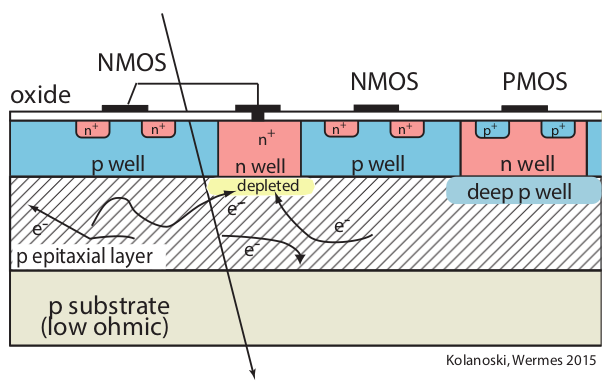
\includegraphics[width=.99\linewidth]{figures/Pixel_detectors/MAPS_scheme.png}
            \column{0.6\textwidth}  
                %\begin{tikzpicture}[overlay]
                %    \draw[decorate,decoration={brace}]
                %        (0,-0.4) -- node[xshift=2pt,anchor=west] {$\lesssim$\SI{5}{\um} electronics}(0,-0.5);
                %\medskip
                %    \draw[decorate,decoration={brace}]
                %        (0,-1) -- node[xshift=2pt,anchor=west] {$\lesssim$\SI{50}{\um} sensor}(0,-1.7);
                %\end{tikzpicture}
                \bigskip
                \begin{equation*}
                    \hspace{75pt} d \propto \sqrt{\rho V}
                \end{equation*}   
                \begin{equation*}
                    %\hspace{75pt} ENC^2 \propto \frac{4}{3} \frac{kT}{g_m} \frac{C_D ^2}{\tau_{sh}}
                    \hspace{75pt} ENC^2 \propto C_D ^2
                \end{equation*}  
                \begin{equation*}
                    %\hspace{75pt} \tau \propto \frac{1}{g_m}\frac{C_D}{C_f}
                    \hspace{75pt} \tau \propto C_D
                \end{equation*}  
            \end{columns} 
        %\begin{equation*}
        %    \hspace{75pt} d \propto \sqrt{\rho V}
        %\end{equation*}     
        \medskip 
        \begin{itemize}
            \item Electronics is low resistivity $\rho$ while sensor needs high $\rho$, special technologies for the sensor. Next slide!  High resistivity allows for depleted epi-layer DMAPS
            \item If not completed depleted charge is collected by diffusion
            \item Very low capacity $\sim$\SI{1}{fF/cm\squared}
            \item epitaxial layer with doping few order of magnitude smaller than the subtrate
        \end{itemize}
    \end{frame} 



    %%%%%%%%%%%%%%%%%%%%%%%%%%%%%%%%%%%%%%%%
    %%  Slide 3: <Sensors types>  %%
    %%%%%%%%%%%%%%%%%%%%%%%%%%%%%%%%%%%%%%%%
    \begin{frame}
        \frametitle{Sensor types}
            \begin{itemize}
                \item Large and small fill factor, depending on the deep p-well structures
            \end{itemize}
            $<$\SI{5}{fF} vs $\sim$100-200\si{fF}, formule ENC e tau

            \centering
            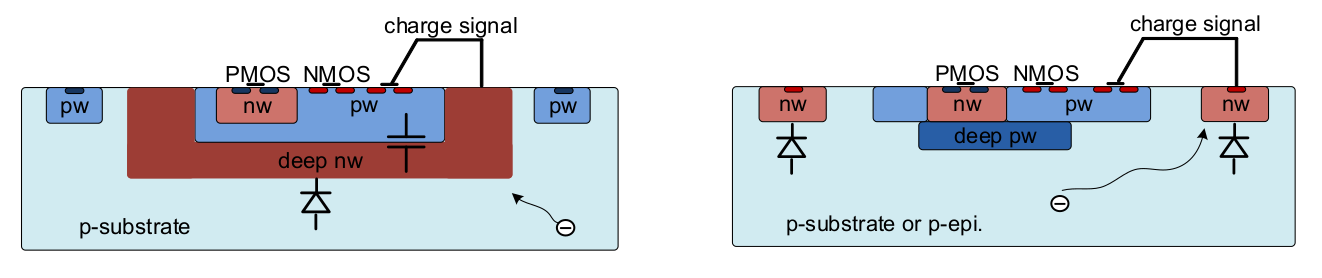
\includegraphics[width=.9\linewidth]{figures/Pixel_detectors/large_small_sensor_scheme.png}\\
            \begin{columns}
                \column{0.5\textwidth}  
                    \centering
                    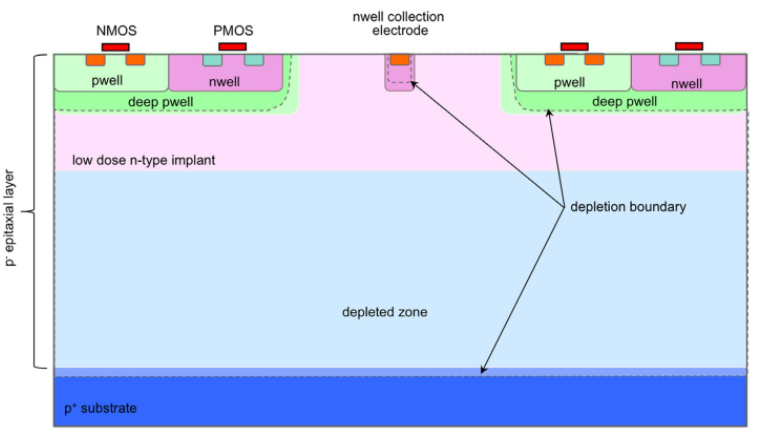
\includegraphics[width=0.8\linewidth]{figures/Pixel_detectors/ALPIDE_after_PM.png}
                \column{0.5\textwidth}  
                    \begin{itemize}
                        \item Process modification with a low dose planar implant \\
                        main investigator ALICE\\
                        no need of change in the sensor and circuit layout
                    \end{itemize} 
            \end{columns}

            \end{frame} 

    %%%%%%%%%%%%%%%%%%%%%%%%%%%%%%%%%%%%%%%%
    %%  Slide 1: <READOUT>  %%
    %%%%%%%%%%%%%%%%%%%%%%%%%%%%%%%%%%%%%%%%
    \begin{frame}
        \frametitle{Front end}
            \begin{columns}
                \column{0.75\textwidth}  
                Pixel area economy and dimension of components are extremely relevant. MAPS usage allowed by miniaturization of components: starting from \SI{600}{nm} down to 120-180{nm} CMOS imaging process of transistors
                \column{0.35\textwidth}  
                    \begin{figure}[h!]
                        \centering
                        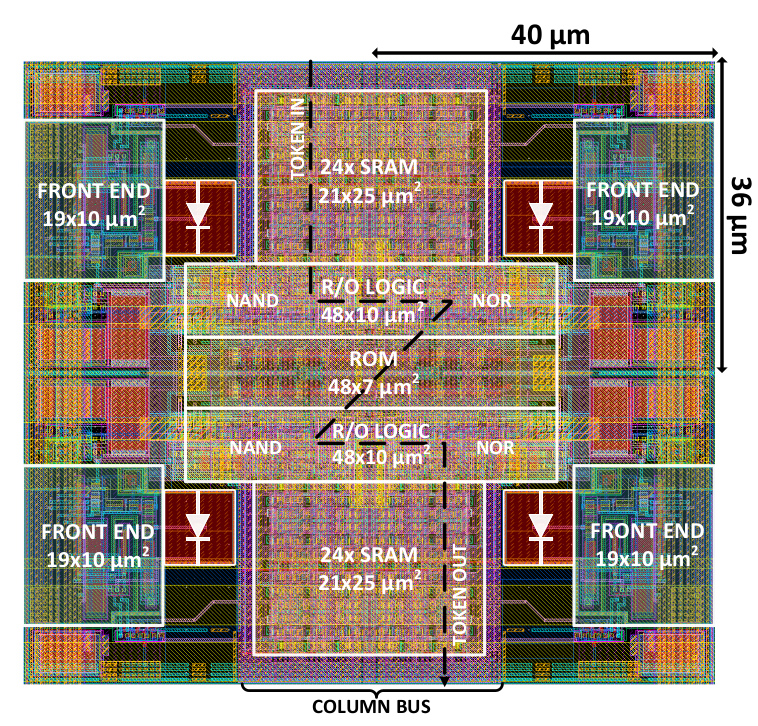
\includegraphics[width=0.99\linewidth]{figures/Monopix1/Monopix1_2x2pixelsgroup.png}
                    \end{figure}
            \end{columns}


        \begin{itemize}
            \item Analog or digital output: ToT is a compromise
            \item Rolling shut or sparsified (data push) readout 
            \item Triggered or triggerless
            \item Column drain is one of the most popular readout mechanism, but other possible are possible
            \item Buffer on pixel to store more than one hit data
        \end{itemize}
 
    \end{frame} 


\begin{frame}[noframenumbering]
    \frametitle{Outline}
    \begin{itemize}
        \item Pixel detectors 
        \item CMOS Monolithic Active Pixels 
        \item <alert@1> TJ-Monopix1
        \begin{enumerate}
            \item TJ-Monopix1 design
            \item TJ-Monopix1 analog output
        \end{enumerate}        
        \item Characterization 
        \item Beam test and FLASH-RT
    \end{itemize}
\end{frame}
\section{TJ-Monopix1}

    %%%%%%%%%%%%%%%%%%%%%%%%%%%%%%%%%%%%%%%%
    %%  Slide 1: <>  %%
    %%%%%%%%%%%%%%%%%%%%%%%%%%%%%%%%%%%%%%%%
    \begin{frame}
        \frametitle{}
        \begin{figure}[h!]
            \centering
            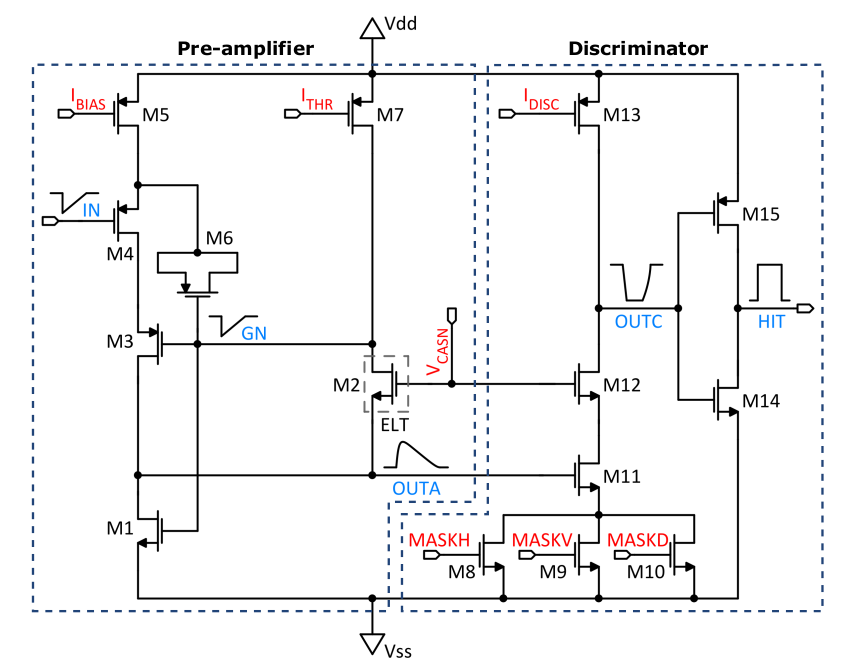
\includegraphics[width=.8\linewidth]{figures/Monopix1/Monopix1_FE_circuit.png}        
        \end{figure}
    \end{frame}     

    %%%%%%%%%%%%%%%%%%%%%%%%%%%%%%%%%%%%%%%%
    %%  Slide 1: <TJ-Monopix1>  %%
    %%%%%%%%%%%%%%%%%%%%%%%%%%%%%%%%%%%%%%%%
    \begin{frame}
        \frametitle{}
        \begin{figure}[h!]
            \centering
            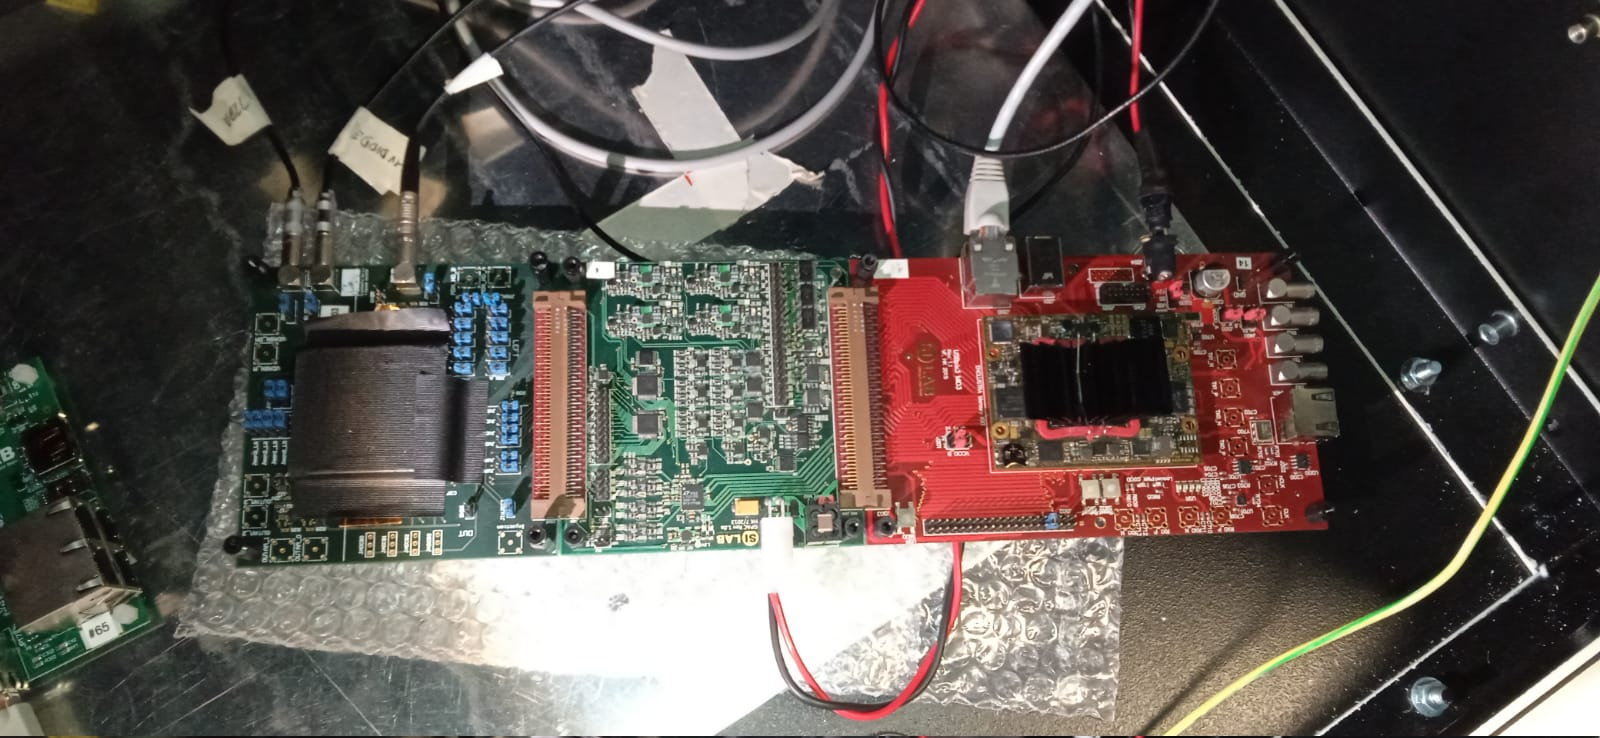
\includegraphics[width=.8\linewidth]{figures/Monopix1/monopix1_front.jpeg}
        \end{figure}

    \end{frame} 



\begin{frame}[noframenumbering]
    \frametitle{Outline}
    \begin{itemize}
        \item Pixel detectors 
        \item CMOS Monolithic Active Pixels 
        \item TJ-Monopix1
        \item <alert@1> Characterization 
        \begin{enumerate}
            \item Threshold and noise
            \item Calibration of the ToT
            \item Characterization with radioactive sources
            \item Study of the readout time
        \end{enumerate}
        \item Beam test and FLASH-RT
    \end{itemize}
\end{frame}
\section{Charaterization}

    %%%%%%%%%%%%%%%%%%%%%%%%%%%%%%%%%%%%%
	%%  Slide 1: <Scurve> %%
	%%%%%%%%%%%%%%%%%%%%%%%%%%%%%%%%%%%%%
    \begin{frame}
        \frametitle{Threshold and noise}
        Injection circuit: at the FE input a charge.
        Charge injected depends on the C$_{inj}$, different for each pixel
        \begin{multicols}{2}
            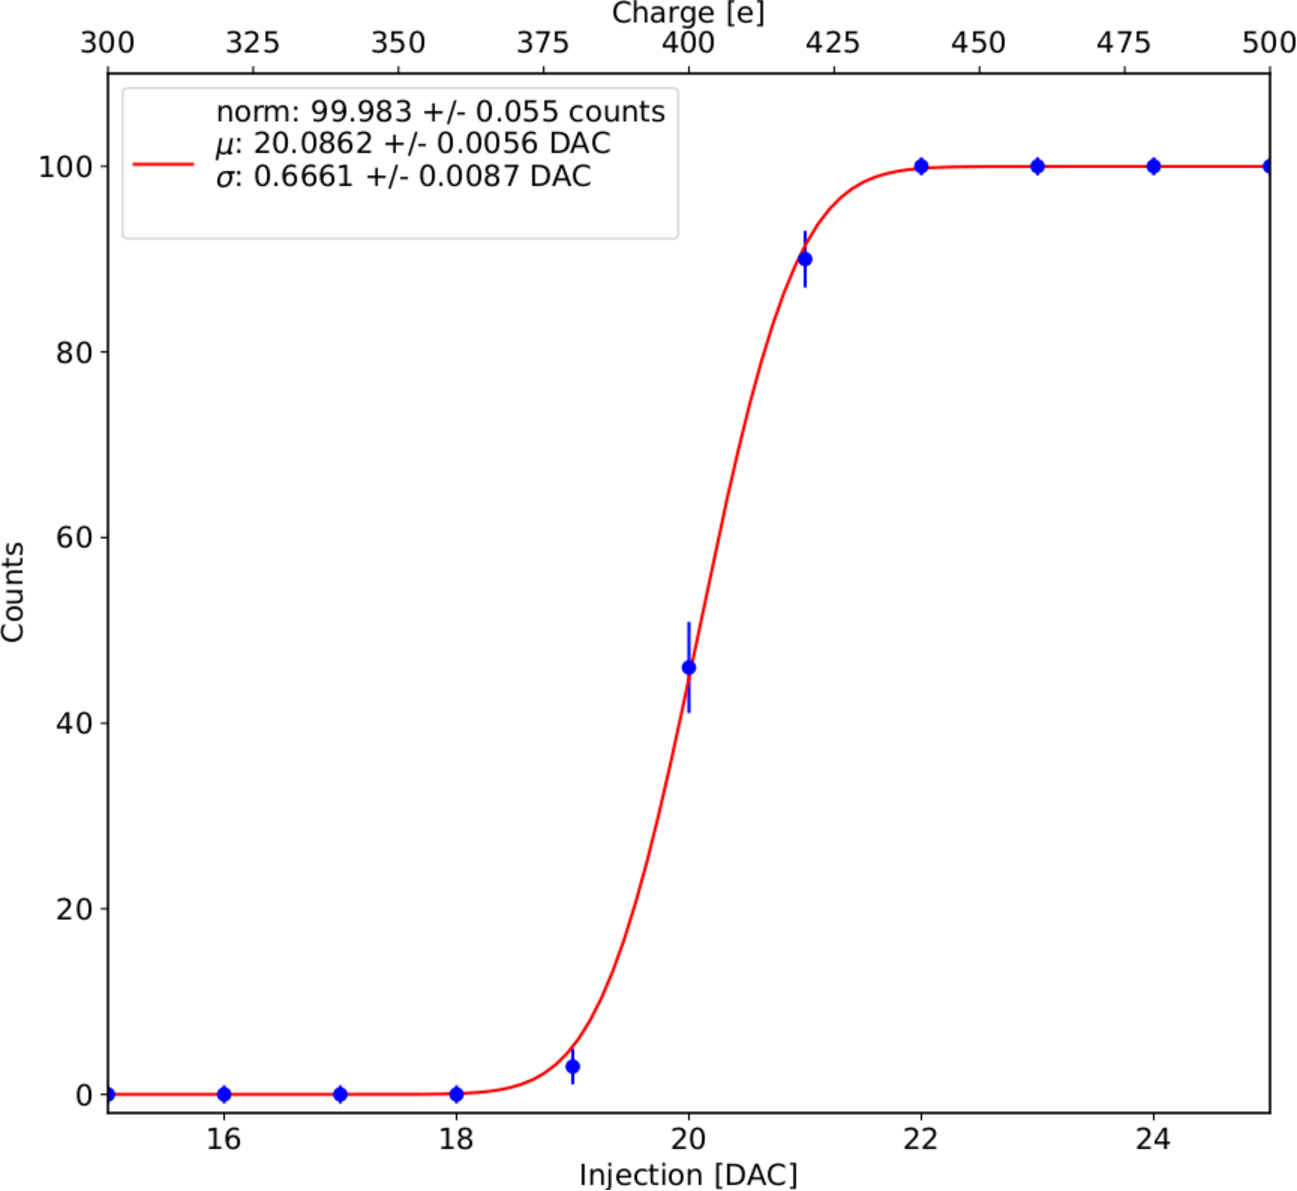
\includegraphics[width=1.\linewidth]{figures/charaterization/scurve.pdf}
        \columnbreak
            \begin{equation}
                erf=
            \end{equation}	
            Assuming a gaussian noise:\\
            threshold=$\mu$ \\
            noise=1/s=$\sigma$
        \end{multicols} 
 
    \end{frame}


    %\begin{center}
    %\end{center}
    
    %%%%%%%%%%%%%%%%%%%%%%%%%%%%%%%%%%%%%%%%
    %%  Slide 2: <Threshold_noise>  %%
    %%%%%%%%%%%%%%%%%%%%%%%%%%%%%%%%%%%%%%%%
    \begin{frame}
        \frametitle{Threshold and noise}
        \begin{figure}[h!]
            \centering
            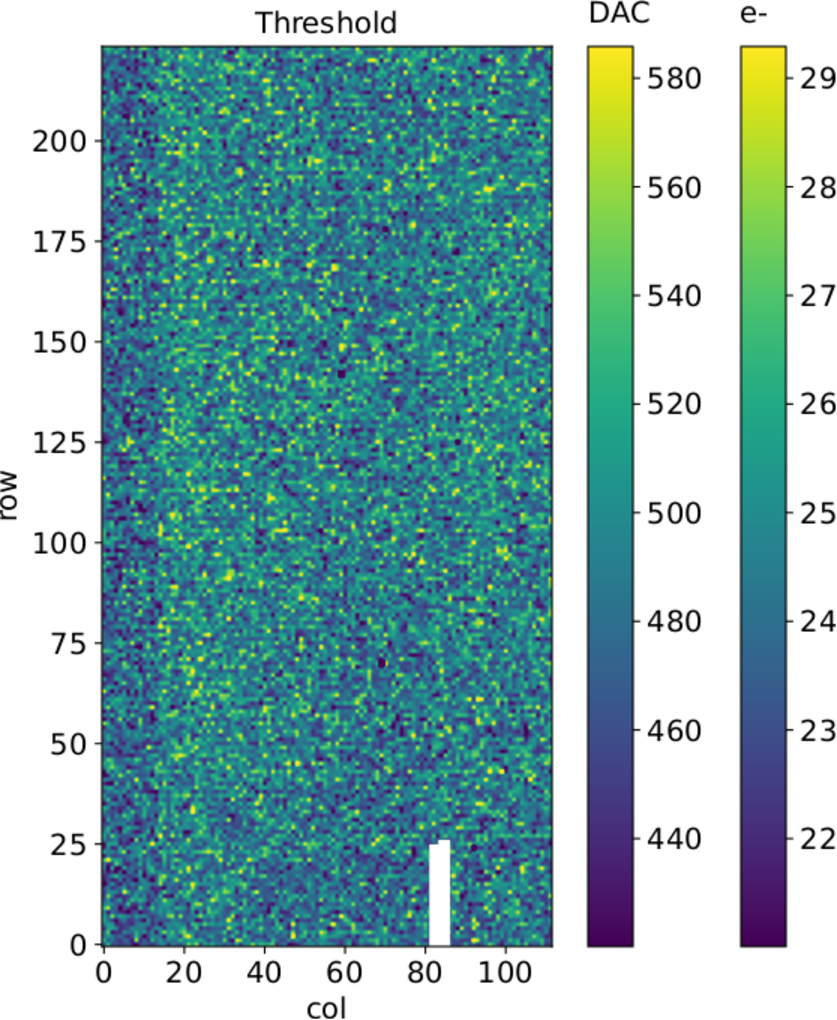
\includegraphics[width=.45\linewidth]{figures/charaterization/threshold_map.pdf}
            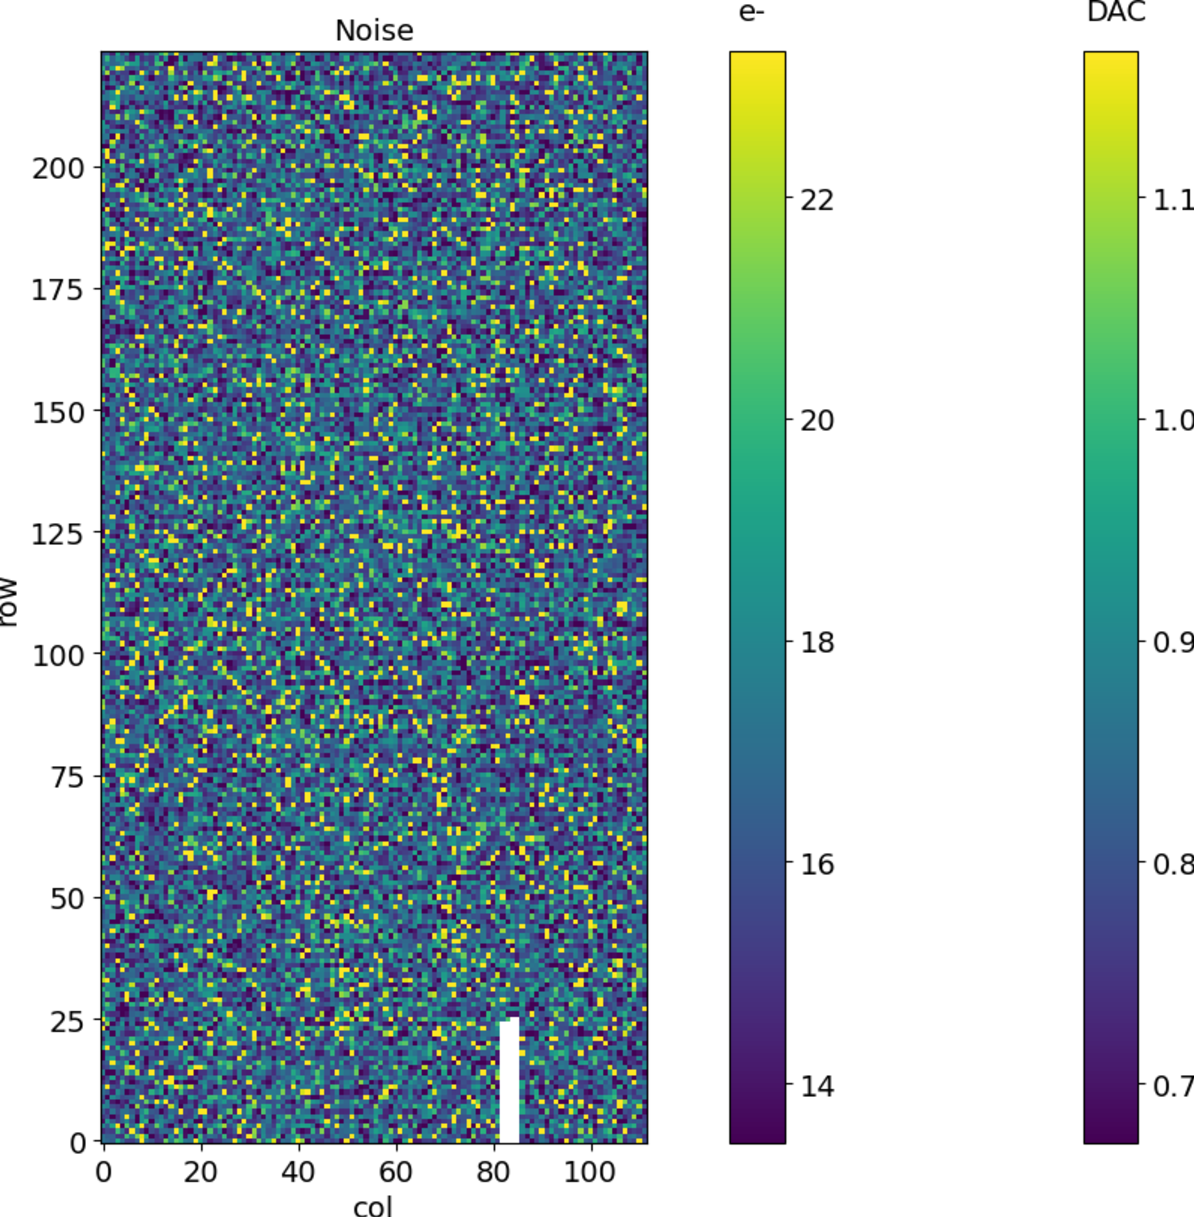
\includegraphics[width=.45\linewidth]{figures/charaterization/noise_map.pdf}
        \end{figure}
        Injection circuit broken
    \end{frame}

    %%%%%%%%%%%%%%%%%%%%%%%%%%%%%%%%%%%%%%%%
    %%  Slide 3: <ToT linearity>  %%
    %%%%%%%%%%%%%%%%%%%%%%%%%%%%%%%%%%%%%%%%
    \begin{frame}
        \frametitle{ToT linearity}
        \begin{itemize}
            \item The ToT linearity is due to the \textbf{PMOS} reset circuit which guaranties the costant discharge in time of the preamplifier (in general is not true)
            \item ToT is saved as a 6-bit variable
        \end{itemize}
        \medskip
        \medskip
        \medskip
        \begin{columns}
            \column{0.6\textwidth}  
                \centering
                Linearity tested with the injection
                \begin{figure}[h!]
                    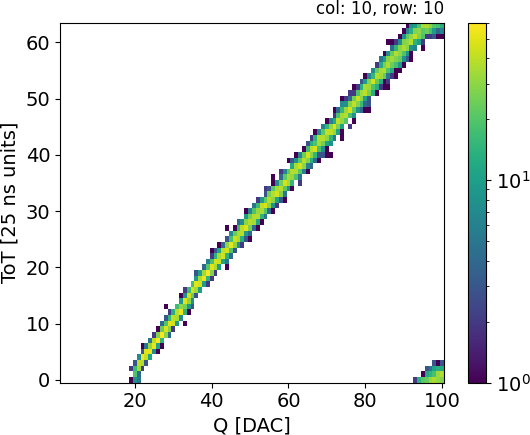
\includegraphics[width=.49\linewidth]{figures/charaterization/ToT_rollover.png}
                    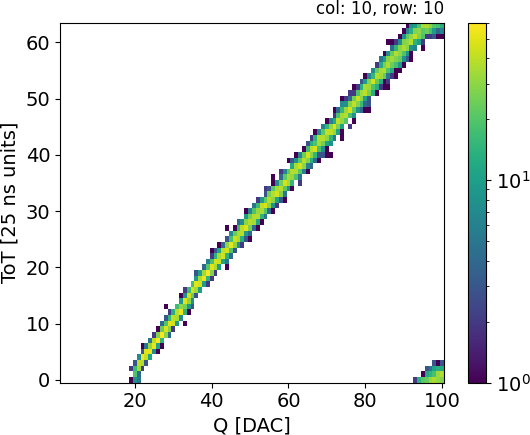
\includegraphics[width=.49\linewidth]{figures/charaterization/ToT_rollover.png} 
                \end{figure}
            \column{0.4\textwidth}
                \textbf{Rollover!}\\
                ToT varies in range 0-63

        \end{columns}
    \end{frame}    

    %%%%%%%%%%%%%%%%%%%%%%%%%%%%%%%%%%%%%%%%
    %%  Slide 4: <ToT vs charge>  %%
    %%%%%%%%%%%%%%%%%%%%%%%%%%%%%%%%%%%%%%%%
    \begin{frame}
        \frametitle{ToT vs charge }
        \begin{beamercolorbox}[sep=0em,wd=0.85\textwidth,ht=1.5ex, dp=0.1ex, rounded=true, center]{lightbluebox}
            Fe$^{55}$ $\rightarrow$ Mn$^{55}$ + K$_\alpha$ (\SI{5.9}{keV}) or K$_\beta$ (\SI{6.5}{keV})
        \end{beamercolorbox}

        \begin{tikzpicture}[overlay]
            \draw[decorate,decoration={brace}]
                (3.5,0) -- (5.5,0);
        \end{tikzpicture}


        with K$_\alpha$:
        \begin{itemize}
            \item $\lambda$=\SI{29}{\um}$\rightarrow$ P$_{abs}$=
            \item $w_i$=\SI{3.6}{eV} in Si @ \SI{300}{\kelvin}$\rightarrow$ \SI{1616}{\elementarycharge}$^-$
        \end{itemize}

        Provide a way 1) to measure the C$_{inj}$ and 2) calibrate the signal

    \end{frame}        

    %%%%%%%%%%%%%%%%%%%%%%%%%%%%%%%%%%%%%%%%
    %%  Slide 4: <ToT calibration>  %%
    %%%%%%%%%%%%%%%%%%%%%%%%%%%%%%%%%%%%%%%%
    \begin{frame}
        \frametitle{ToT calibration}
            \begin{figure}[h!]
                \centering
                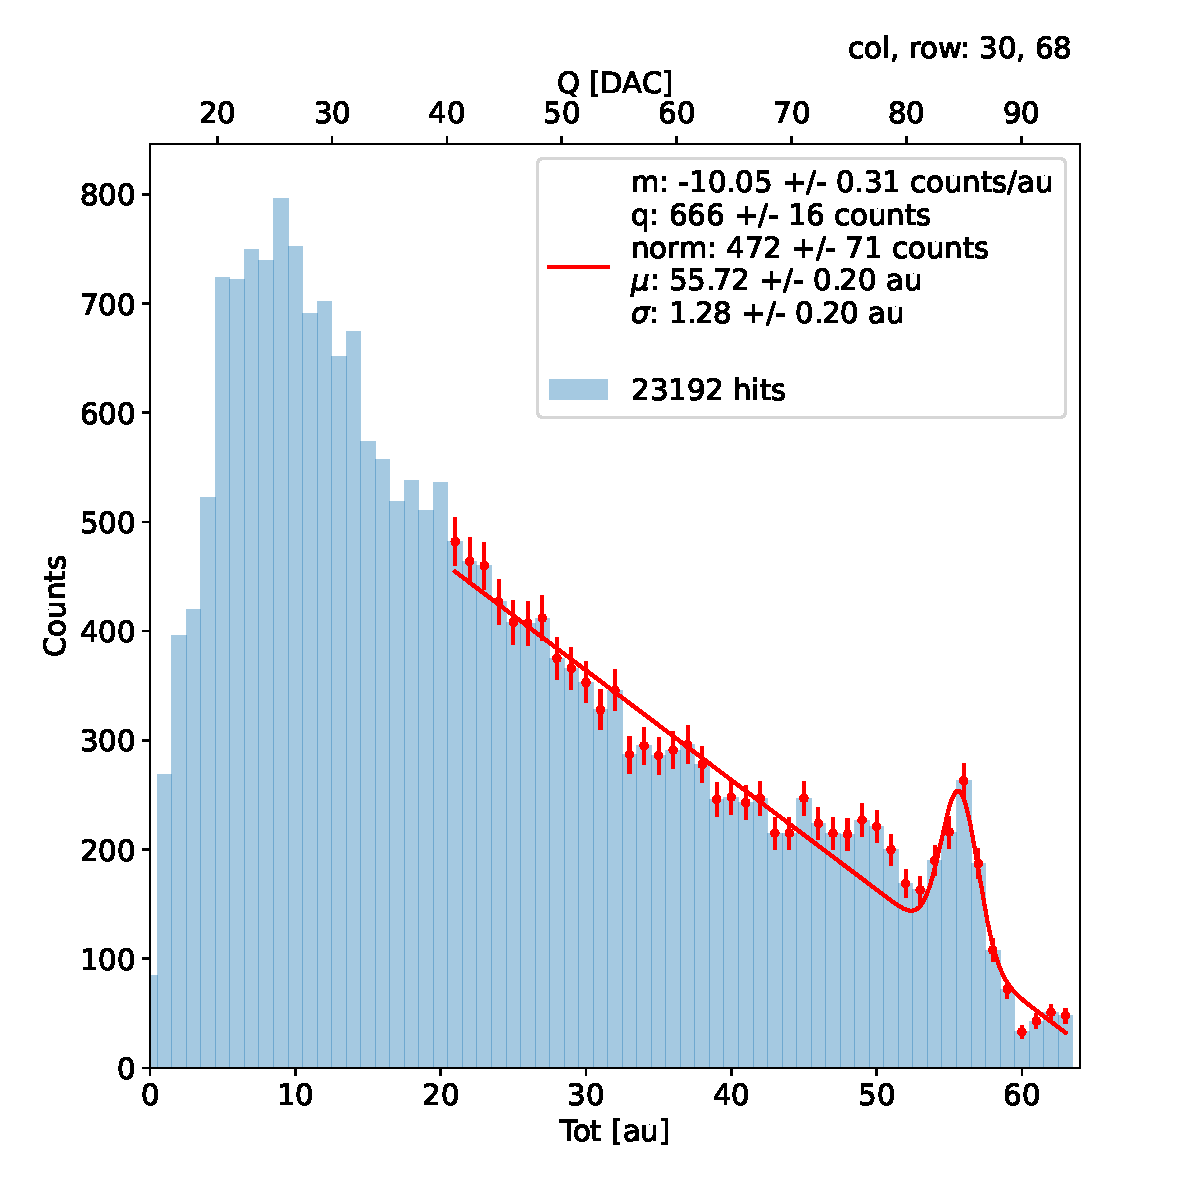
\includegraphics[width=.99\linewidth]{figures/charaterization/fit_line_gauss_r69.pdf}
            \end{figure}

    \end{frame}     


    %%%%%%%%%%%%%%%%%%%%%%%%%%%%%%%%%%%%%%%%
    %%  Slide 5: <ToT bias>  %%
    %%%%%%%%%%%%%%%%%%%%%%%%%%%%%%%%%%%%%%%%
    \begin{frame}
        \frametitle{Bias}
        \begin{figure}[h!]
            \centering
            %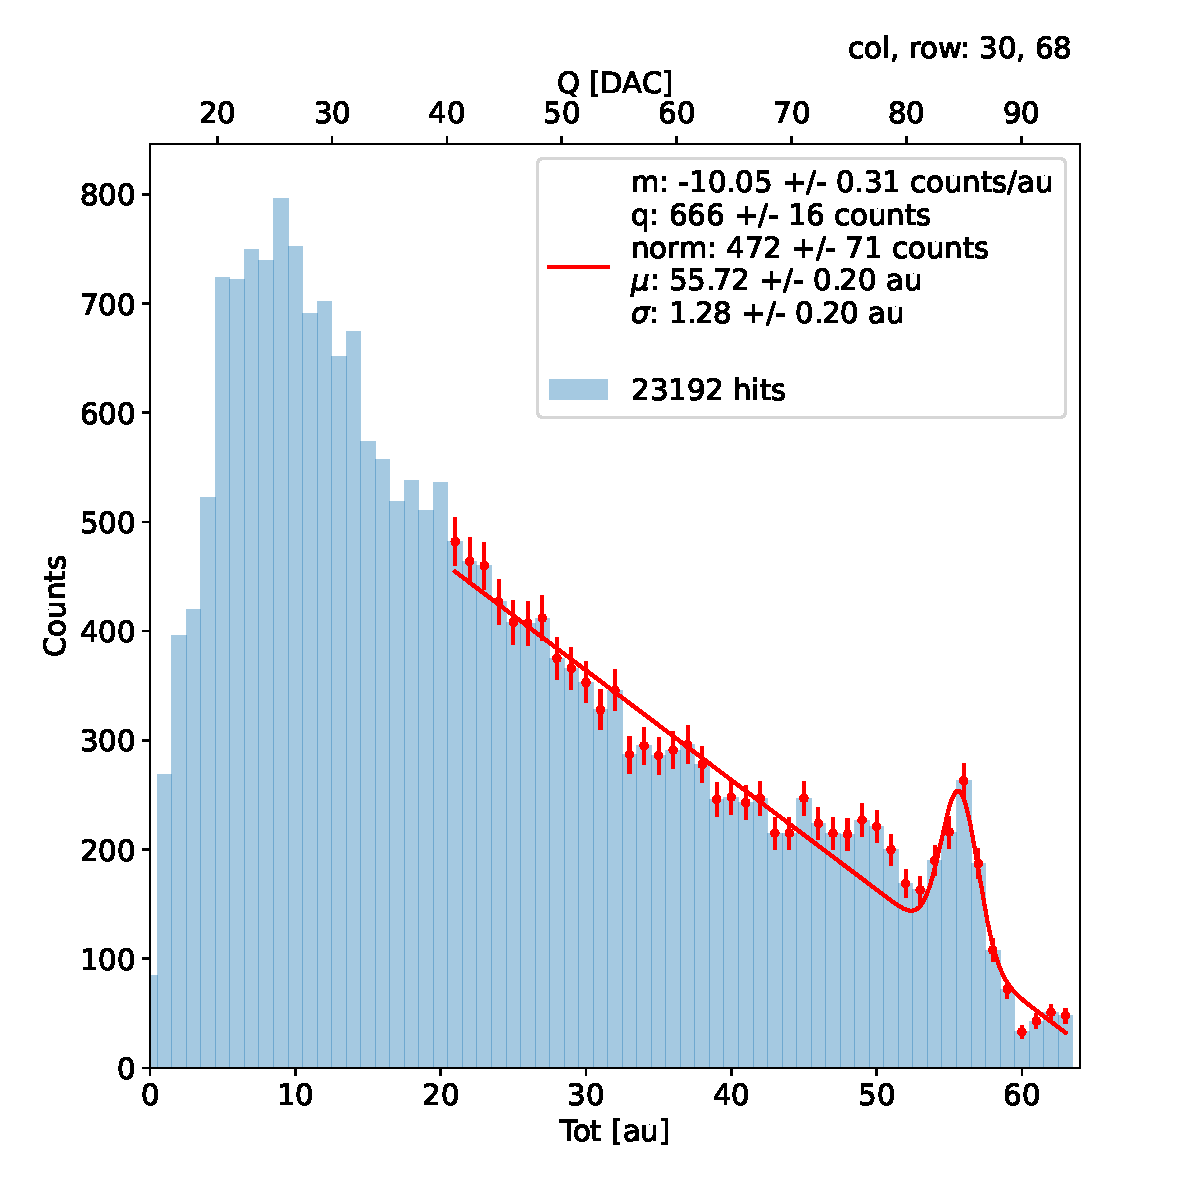
\includegraphics[width=.2\linewidth]{figures/charaterization/fit_line_gauss_r69.pdf}
        \end{figure}
    \end{frame}      

    %%%%%%%%%%%%%%%%%%%%%%%%%%%%%%%%%%%%%%%%
    %%  Slide 5: <Dead time>  %%
    %%%%%%%%%%%%%%%%%%%%%%%%%%%%%%%%%%%%%%%%
    \begin{frame}
        \frametitle{Readout time}
        \begin{figure}[h!]
            \centering
            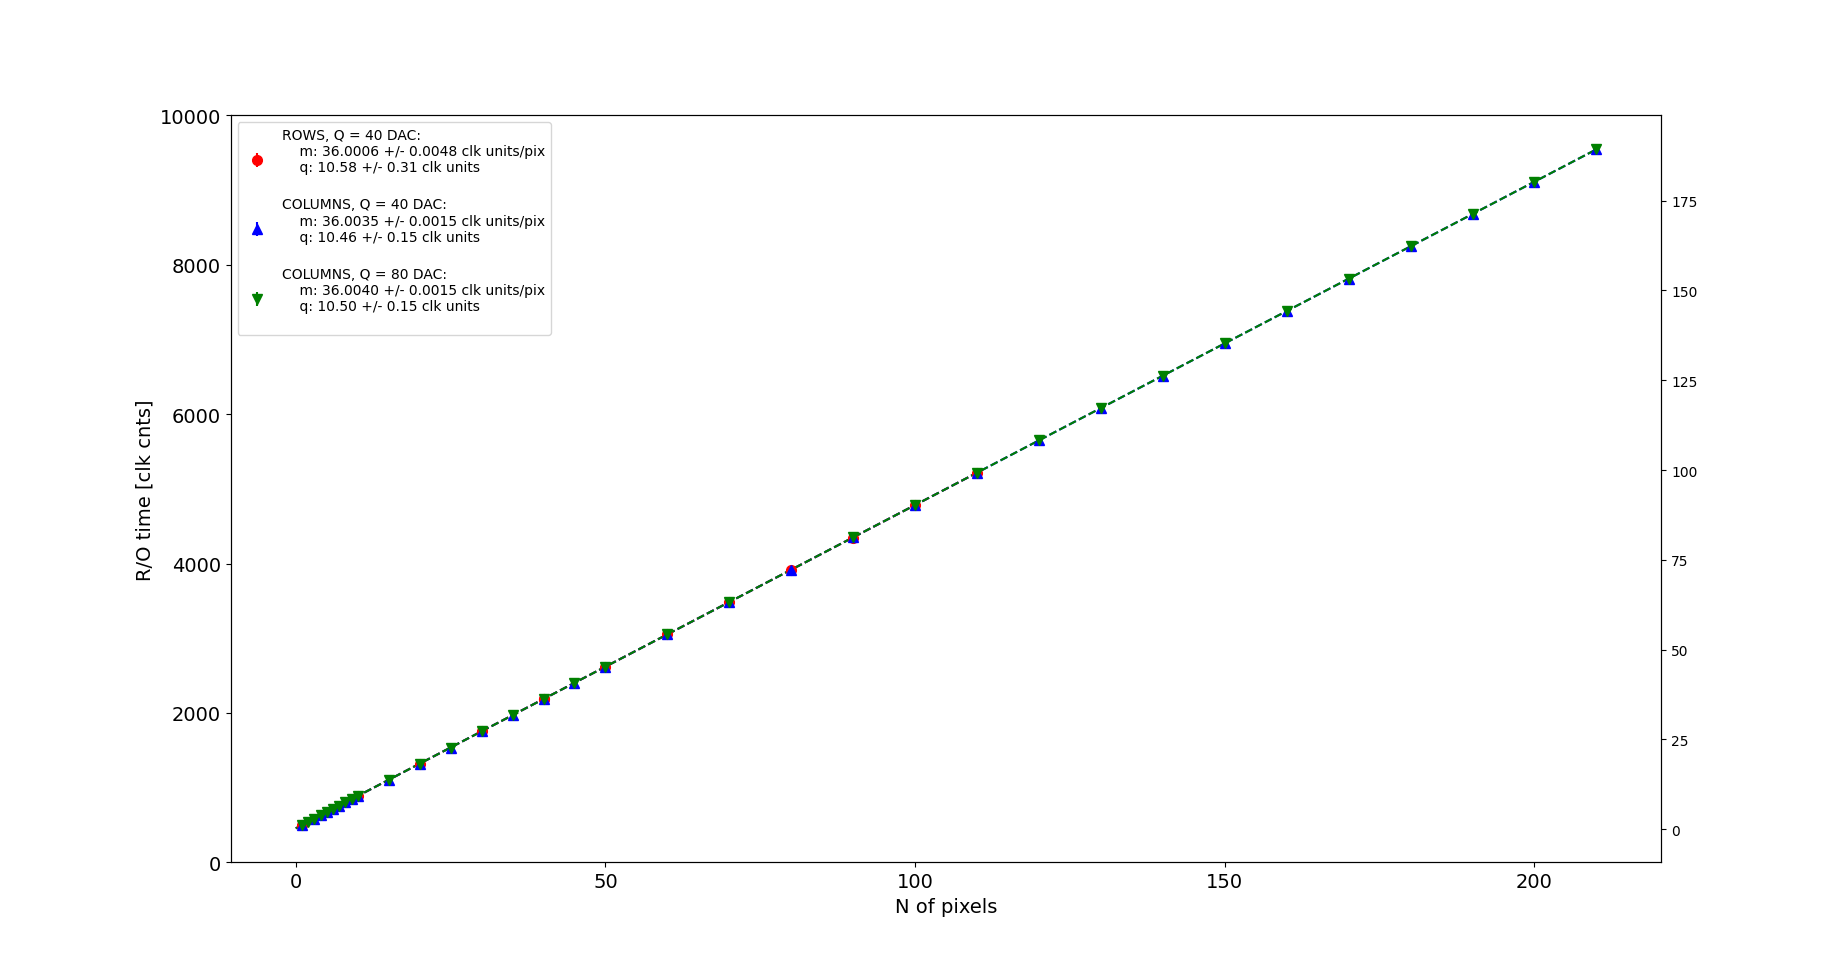
\includegraphics[width=.2\linewidth]{figures/charaterization/default_line.png}
        \end{figure}
    \end{frame}          

\begin{frame}[noframenumbering]
    \frametitle{Outline}
    \begin{itemize}
        \item Pixel detectors 
        \item CMOS Monolithic Active Pixels 
        \item TJ-Monopix1
        \item Characterization 
        \item <alert@1> Beam test and FLASH-RT
        \begin{enumerate}
            \item Motivation: FLASH radiotherapy
            \item Possible application of MAPS in FLASH-RT 
            \item Test on the beam: experimental setup
            \item Test on the beam: preliminary results
        \end{enumerate}
    \end{itemize}
\end{frame}
\section{FLASH-RT}

    %%%%%%%%%%%%%%%%%%%%%%%%%%%%%%%%%%%%%%%%
    %%  Slide 1: <>  %%
    %%%%%%%%%%%%%%%%%%%%%%%%%%%%%%%%%%%%%%%%
    \begin{frame}
        \frametitle{FLASH radiotherapy}
        \begin{itemize}
            \item Radiotherapy takes advantage of the damage caused by the ionization of energy loss by particles
            \item FLASH-RT consists in delivering a high level of dose in a small fraction of time: this seems reducing the toxiticy of the radiation on healty tissues
        \end{itemize}
        \medskip
        \begin{columns}
            \column{0.5\textwidth}  
                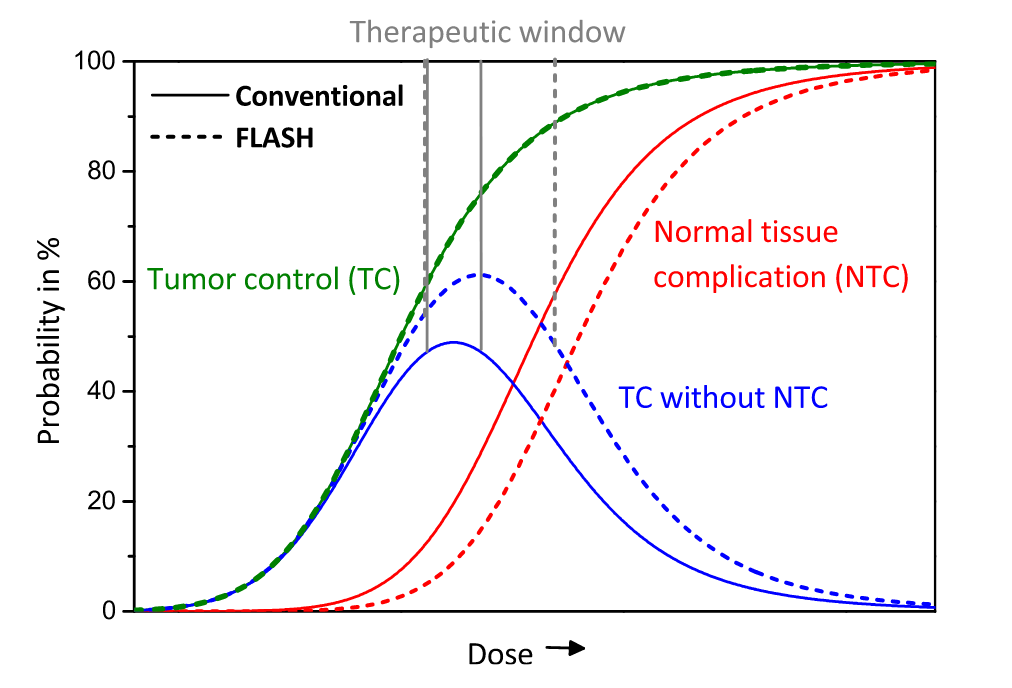
\includegraphics[width=1.25\linewidth]{figures/pixel_detectors_usage/curve_flash.png}
        \column{0.5\textwidth}
            
            \begin{itemize}
                \item FLASH-RT is still \textbf{under test}!
                \begin{itemize}
                    \item medical aspect%: in vitro and with animals; only one patient has been treated
                    \item  bio-physics aspect%: dependence of the FLASH effect on the treatment conditions 
                    \item  strumental aspect%: need for new detectors
                \end{itemize}
            \end{itemize}
        \end{columns}
    \end{frame} 


    %%%%%%%%%%%%%%%%%%%%%%%%%%%%%%%%%%%%%%%%
    %%  Slide 1: <>  %%
    %%%%%%%%%%%%%%%%%%%%%%%%%%%%%%%%%%%%%%%%
    \begin{frame}
        \frametitle{Electron FLASH radiotherapy}
        \centering
        \bigskip
        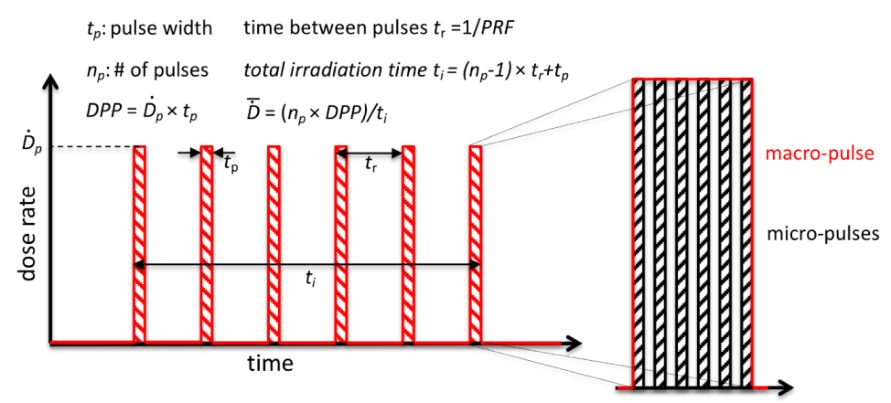
\includegraphics[width=.9\linewidth]{figures/test_beam/beam_structure.pdf}
        \begin{columns}
            \column{0.8\textwidth}
                \begin{table}
                    \footnotesize
                    \begin{center}
                    \begin{tabular}{|c | c |c |}
                    \hline
                    & CONV-RT & FLASH-RT \\
                    \hline
                    \hline
                    Dose rate & \SI{0.03}{Gy/s} & \SI{40}{Gy/s}\\
                    Intra pulse dose rate & \SI{100}{Gy/s}&\SI{10 6}{Gy/s}\\
                    Treatment duration & $\sim$minutes & $\lessapprox$\SI{500}{ms} \\
                    Dose Per Pulse & \SI{0.3}{Gy} & 1-10 Gy\\
                    Pulse width & \SI{3}{\us} & $\sim$\SI{2}{\us} \\
                    \hline
                    \end{tabular}
                    \end{center}
                \end{table} 
                
            \column{0.3\textwidth}
                Assuming \textbf{water} as the dosimetric reference material 
                %\begin{equation*}
                %    N_A[/\si{\cm\squared}] = \frac{DPP[Gy]}{10^{10} S[\si{MeV \cm \squared /g}]}
                %\end{equation*}
        \end{columns}
    \end{frame}     


    %%%%%%%%%%%%%%%%%%%%%%%%%%%%%%%%%%%%%%%%
    %%  Slide 1: <dosimeters>  %%
    %%%%%%%%%%%%%%%%%%%%%%%%%%%%%%%%%%%%%%%%
    \begin{frame}
        \frametitle{FLASH-RT: need for detectors}
        All online detector types show saturation problems at such high intensity
        \medskip
        \begin{columns}
            \column{0.4\textwidth} 
            Different types of detector with different charateristics are required: 
                \begin{itemize}
                    \item \textbf{dosimeters} 
                    \item \textbf{beam monitors} 
                    \item detectors for diagnostic 
                \end{itemize}
            \column{0.6\textwidth}  
                \hspace*{-0.6cm}
                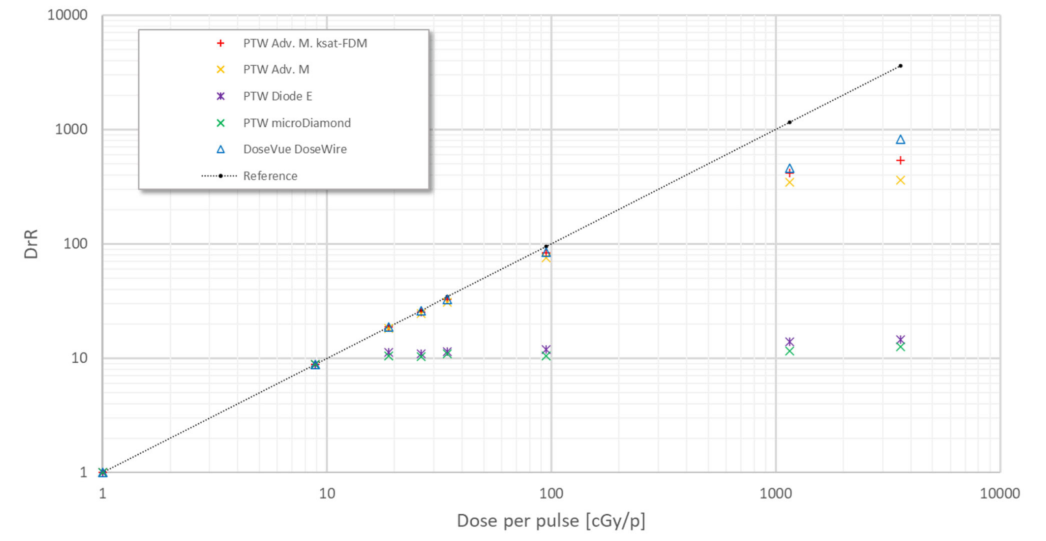
\includegraphics[width=1.15\linewidth]{figures/pixel_detectors_usage/saturation_dosimeters.pdf}
                %COSA SONO I COLORI
                Rif.articolo\\\bigskip
                \hspace*{-3.cm}$N_A$ = 0.2-1.2 10$^9$/cm$^2$ @ Dose Per Pulse = 0.07-0.4 Gy
        \end{columns}
    \end{frame}     



    %%%%%%%%%%%%%%%%%%%%%%%%%%%%%%%%%%%%%%%%
    %%  Slide 1: <dosimeters>  %%
    %%%%%%%%%%%%%%%%%%%%%%%%%%%%%%%%%%%%%%%%
    \begin{frame}
        \frametitle{Possible applications of MAPS}
        \begin{enumerate}
            \item \textbf{Dosimeters}: very difficult because of saturation effect. \\
            Need to: 
            \begin{itemize}
                \item divide the charge of one pulse in microbuckets
                \item reduce the FE charge sensitivity by large factor 
                \item use a fast FE and a fast readout
            \end{itemize}
            \bigskip
            \item \textbf{Beam position monitors}: very thin detectors ($\sim$\SI{50}{\um}) with low disturbance 
                \begin{itemize}
                    \item \textbf{Very High Energy Electrons FLASH-RT} that uses pencil beams, in this case the pixels are saturated but it does not matter
                \end{itemize}
        \end{enumerate}
    \end{frame}     


    %%%%%%%%%%%%%%%%%%%%%%%%%%%%%%%%%%%%
    %% Slide 2: <> %%
    %%%%%%%%%%%%%%%%%%%%%%%%%%%%%%%%%%%%
    \begin{frame}
        \frametitle{Test on the beam: experimental set up}
        \smallskip
        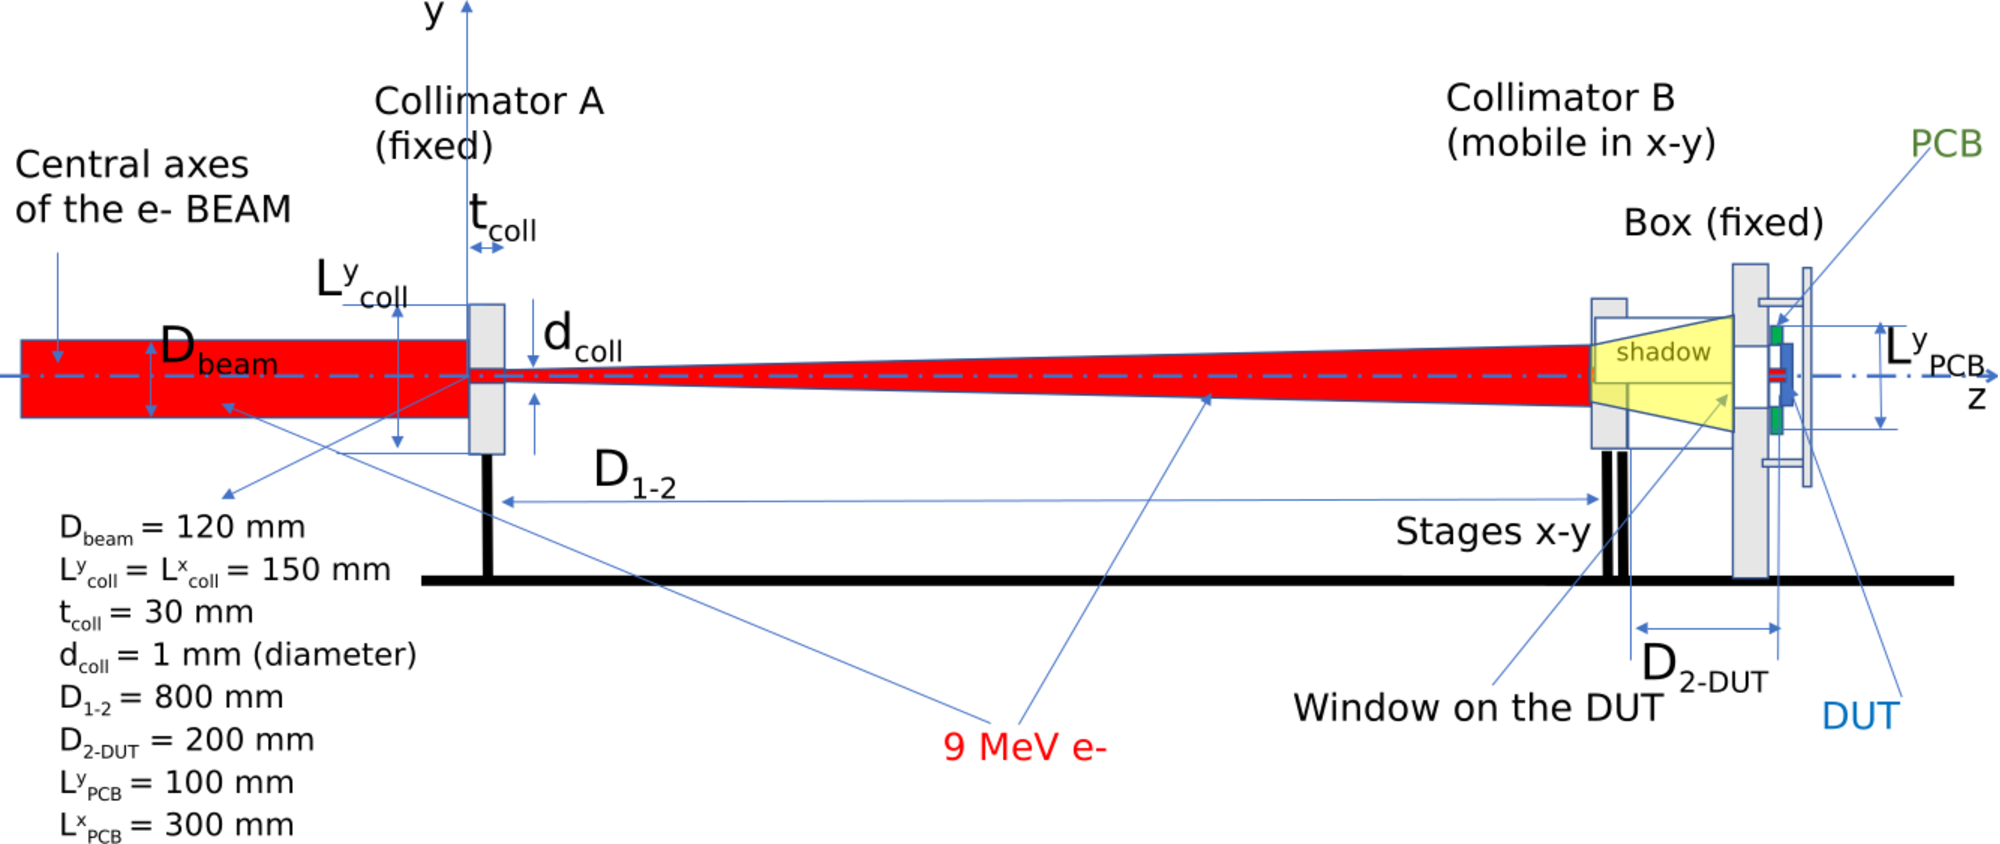
\includegraphics[width=.95\linewidth]{figures/test_beam/Flash-beam-scheme.pdf}\\
        \smallskip
        \begin{enumerate}
            \item Collimator A: to reduce fluence on the DUT of \textbf{4 10$^{-4}$}
            \item Collimator B: to illuminate only a small portion of DUT to see the beam border
        \end{enumerate}
        %$N_A$ = 2.9 10$^9$/cm, F = 7.25$\times$10$^{9}$\si{MHz/cm\squared} @  DPP=\SI{1}{Gy}, t$_p$=\SI{4}{\us}
        
    \end{frame}    


    %%%%%%%%%%%%%%%%%%%%%%%%%%%%%%%%%%%%
    %% Slide 2: <> %%
    %%%%%%%%%%%%%%%%%%%%%%%%%%%%%%%%%%%%
    \begin{frame}
        \frametitle{Test on the beam: experimental set up}
        \centering
        \includegraphics[width=.7\linewidth]{figures/test_beam/testbeam_photos.pdf}  
    \end{frame}    

    %%%%%%%%%%%%%%%%%%%%%%%%%%%%%%%%%%%%
    %% Slide 2: <> %%
    %%%%%%%%%%%%%%%%%%%%%%%%%%%%%%%%%%%%
    \begin{frame}
        \frametitle{Test on the beam: preliminary results}
        \begin{columns}
            \column{0.5\textwidth} 
                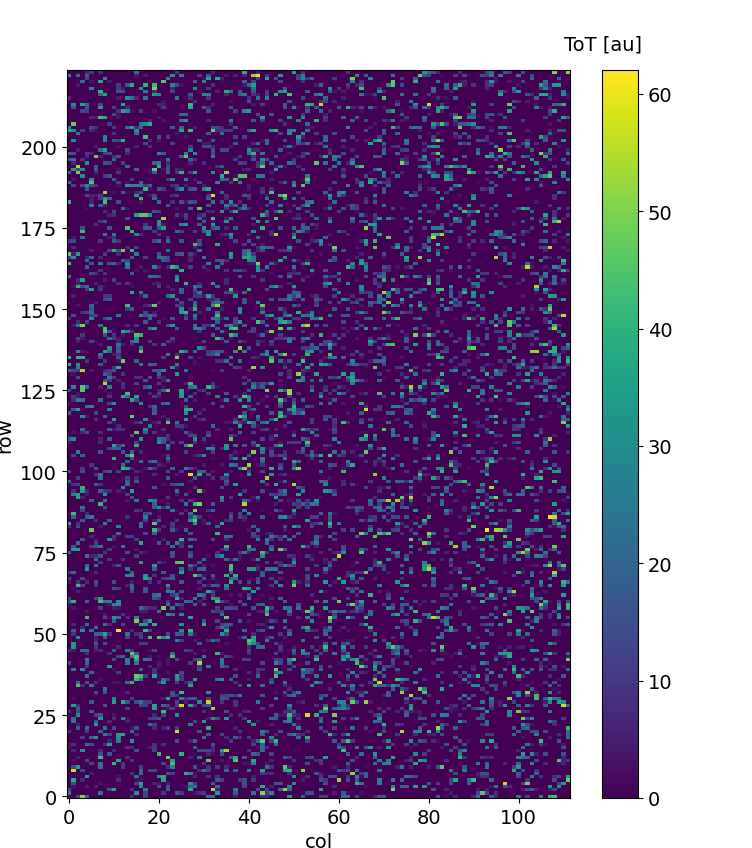
\includegraphics[width=1.1\linewidth]{figures/test_beam/tot_mapq1_15-57.png}  
            \column{0.5\textwidth} 
                \begin{itemize}
                    \item Under-extimation of the Bremsstrahlung production of electrons which stop in the collimators 
                    \item High background in data
                    \item Need for a simulation to better understand the data
                \end{itemize}
            \end{columns}
        \end{frame}  


    %%%%%%%%%%%%%%%%%%%%%%%%%%%%%%%%%%%%
    %% Slide 2: <> %%
    %%%%%%%%%%%%%%%%%%%%%%%%%%%%%%%%%%%%
    \begin{frame}
        \frametitle{Test on the beam: preliminary results}
        \begin{columns}
            \column{0.5\textwidth} 
                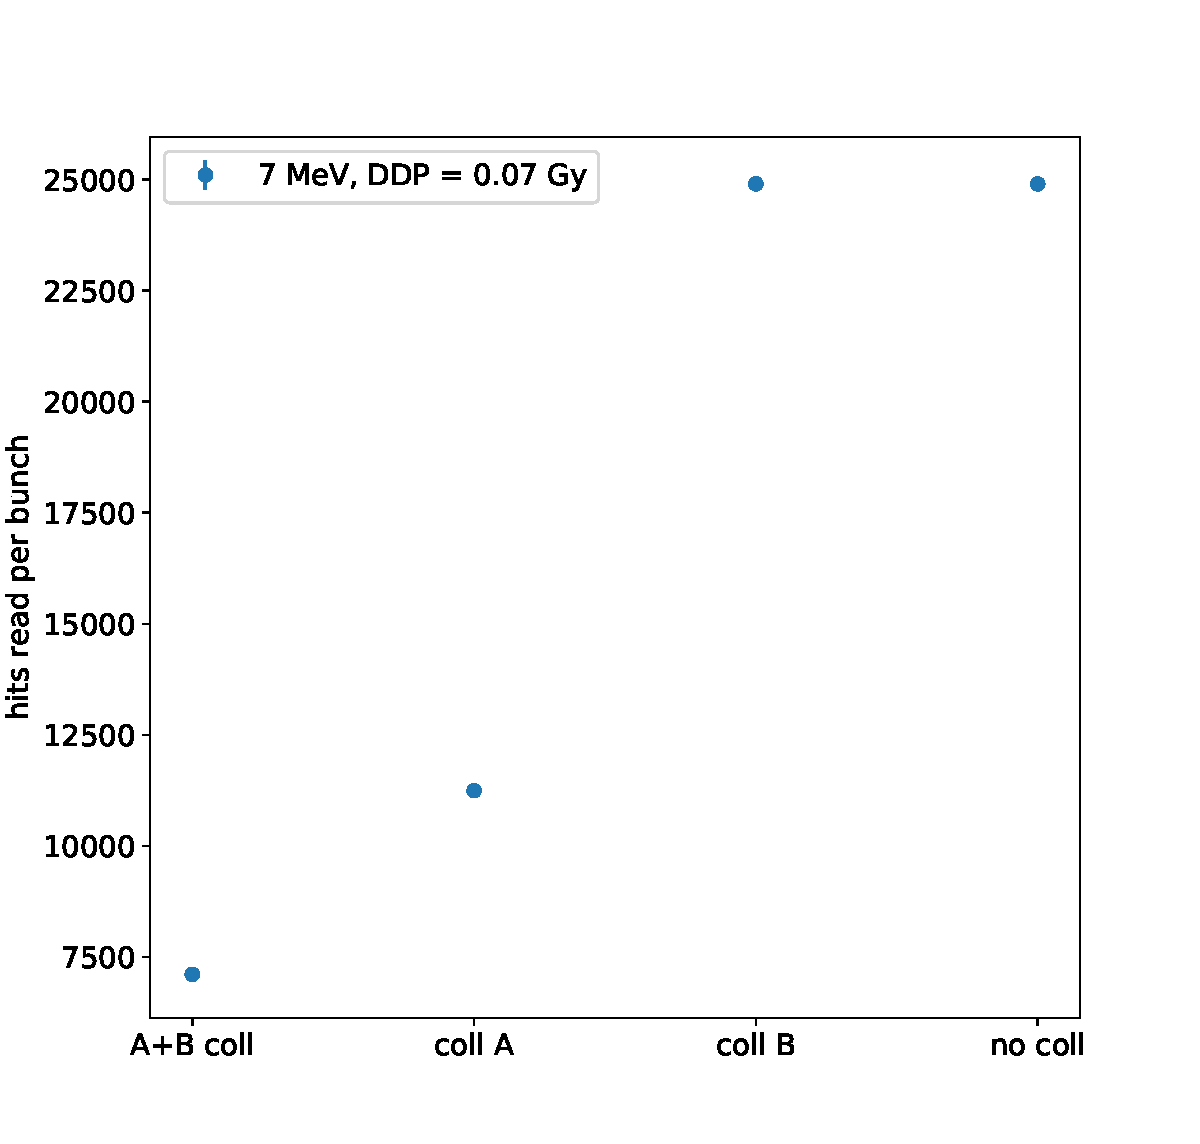
\includegraphics[width=1.1\linewidth]{figures/test_beam/hits.pdf}  
            \column{0.5\textwidth} 
                \begin{itemize}
                    \item Saturation due to the readout system occurs without collimators
                    \item Readout logic has been tested with high hit rate
                \end{itemize}
            \end{columns}
        \end{frame}  

\input{presentation/conclusions.tex}

    %%%%%%%%%%%%%%%%%%%%%%%%%%%%%%%%%%%%%%%%
    %%  Slide 1: <BACKUP>  %%
    %%%%%%%%%%%%%%%%%%%%%%%%%%%%%%%%%%%%%%%%
    \begin{frame}
        Backup        
    \end{frame} 

    

    %%%%%%%%%%%%%%%%%%%%%%%%%%%%%%%%%%%%%%%%
    %%  Slide 1: <>  %%
    %%%%%%%%%%%%%%%%%%%%%%%%%%%%%%%%%%%%%%%%
    \begin{frame}
        \frametitle{}
        \begin{figure}[h!]
            \centering
            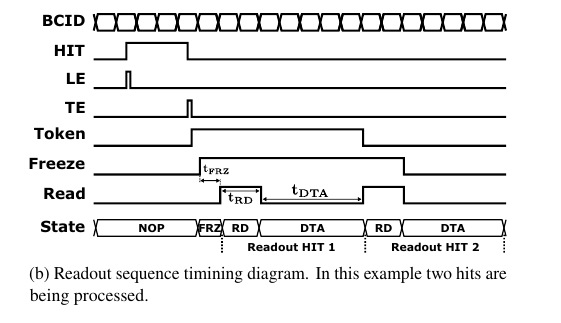
\includegraphics[width=.8\linewidth]{figures/Monopix1/readout_timing.png}
        \end{figure}
    \end{frame} 

    %%%%%%%%%%%%%%%%%%%%%%%%%%%%%%%%%%%%%%%%
    %%  Slide 1: <>  %%
    %%%%%%%%%%%%%%%%%%%%%%%%%%%%%%%%%%%%%%%%
    \begin{frame}
        \frametitle{Radiotherapy}
        \begin{figure}[h!]
            \centering
            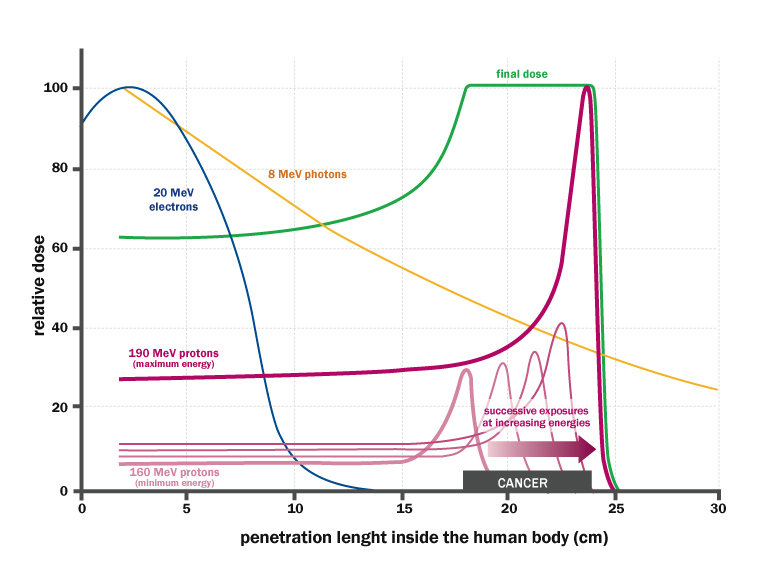
\includegraphics[width=.8\linewidth]{figures/pixel_detectors_usage/Bragg-Peak.png}
        \end{figure}
    \end{frame} 


     %%%%%%%%%%%%%%%%%%%%%%%%%%%%%%%%%%%%%%%%
    %%  Slide 1: <>  %%
    %%%%%%%%%%%%%%%%%%%%%%%%%%%%%%%%%%%%%%%%
    \begin{frame}
        \frametitle{Front end}
            \textbf{ALPIDE like}
            \begin{figure}[h!]
                \centering
                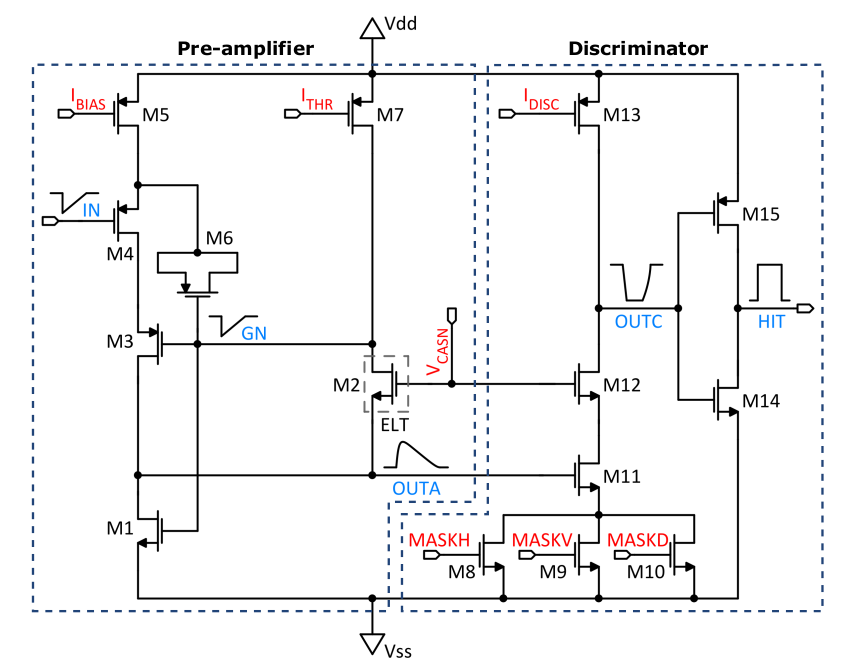
\includegraphics[width=.8\linewidth]{figures/Monopix1/Monopix1_FE_circuit.png}        
            \end{figure}
    \end{frame}     


    %%%%%%%%%%%%%%%%%%%%%%%%%%%%%%%%%%%%%%%%
    %%  Slide 1: <>  %%
    %%%%%%%%%%%%%%%%%%%%%%%%%%%%%%%%%%%%%%%%
    \begin{frame}
        \frametitle{Noisy pixels}
        \begin{columns}
            \column{0.4\textwidth} 
                \centering
                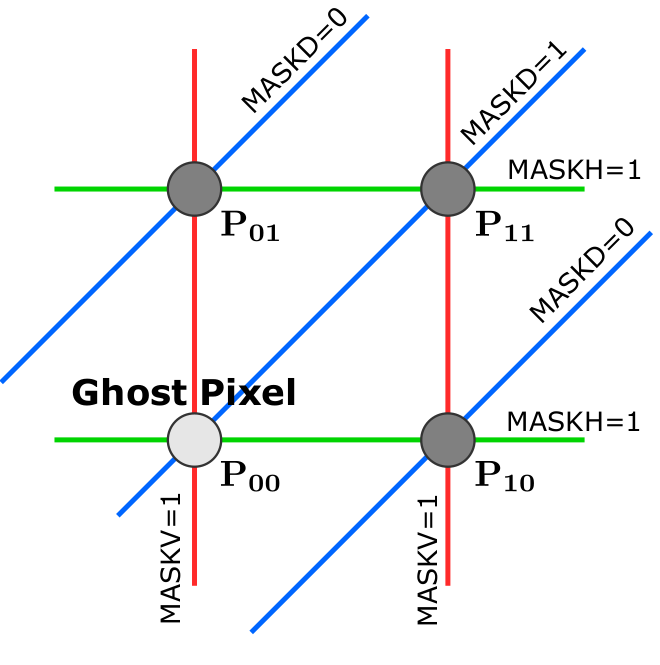
\includegraphics[width=.8\linewidth]{figures/Monopix1/masking_scheme.png}        
            \column{0.4\textwidth} 
            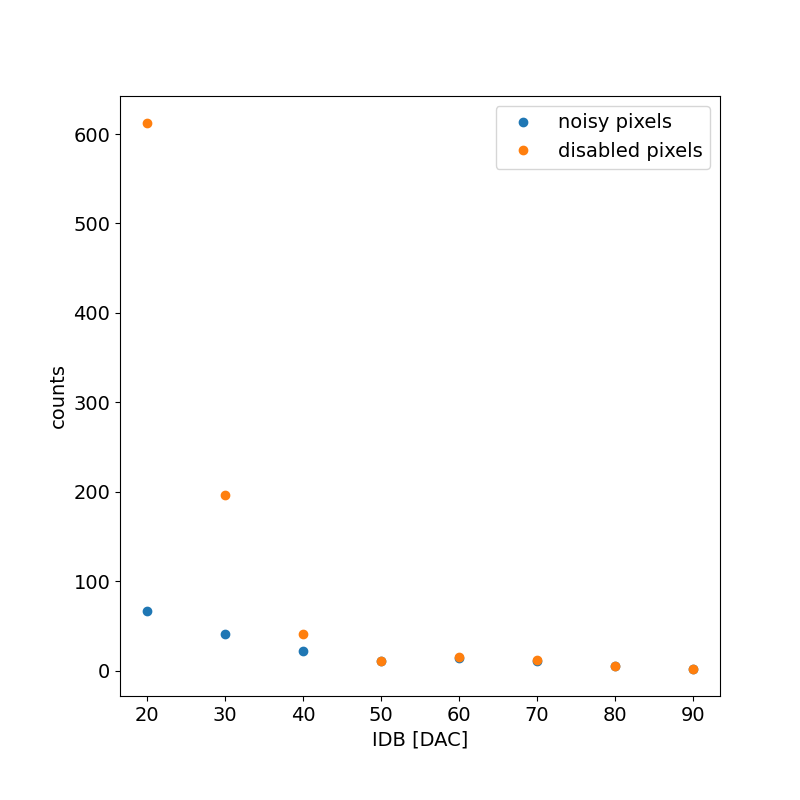
\includegraphics[width=.8\linewidth]{figures/characterization/noisy.png}
        \end{columns}
    \end{frame}    

        
\end{document}